\chapter{Numerical experiments}
\section{Generative modelling experiments}
\subsection{Toy 2D datasets}
For toy 2D experiments we compare Wasserstein GAN with gradient penalty and direct application of topology divergence only. The underlying network is the same MLP across setups. Fitness of distributions is evaluated via k-means cluster and subsequent histogram comparison, providing us with number of statistically different bins \cite{richardson2018gans}, precision-recall curve \cite{sajjadi2018assessing}, Jensen-Shannon divergence and total variation distance.
\begin{table}[h!]
    \centering
    \begin{tabular}{|c|c|}
    \hline
        hidden dim  & 16 \\
        input/output dim & 2 \\
        \# layers & 5 \\
        activation & ReLU \\
    \hline
    \end{tabular}
    \caption{Generator network parameters}
    \label{tab:my_label}
\end{table}

\begin{table}[h!]
    \centering
    \begin{tabular}{||c|c||c|c|c|c||}
        \hline \hline
         Method & Dataset & NDB ratio $\downarrow$& JS $\downarrow$ & max$F_1$ $\uparrow$ & TVD $\downarrow$\\ \hline \hline
         WGAN-GP & 4 Gaussians  & 0.91 & 0.617 & 0.058 & 0.723 \\ \hline
         MTop-Div${}_0$ & 4 Gaussians  & \textbf{0.08} & \textbf{0.0347} & \textbf{0.788} & \textbf{0.015} \\ \hline \hline
         WGAN-GP & 12 Gaussians  & 0.97 & 0.68 & 0.008 & 0.996 \\ \hline
         MTop-Div${}_0$ & 12 Gaussians  & \textbf{0.17} & \textbf{0.058} & \textbf{0.747} & \textbf{0.253} \\ \hline \hline
         WGAN-GP & Moons  & 0.99 & 0.66 & 0.024 & 0.988\\ \hline
         MTop-Div${}_0$ & Moons  & \textbf{0.12} & \textbf{0.047} & \textbf{0.759} & \textbf{0.017} \\ \hline \hline
         WGAN-GP & Swiss Roll  & 0.97 & 0.6 & 0.081 & 0.441 \\ \hline
         MTop-Div${}_0$ & Swiss Roll  & \textbf{0.12} & \textbf{0.034} & \textbf{0.801} & \textbf{0.015} \\ \hline
        \hline
    \end{tabular}
    \caption{Best metrics across toy datasets}
    \label{tab:my_label}
\end{table}

\begin{figure}[h!]
\begin{tabular}{ccc}
\subfloat[Generative sample]{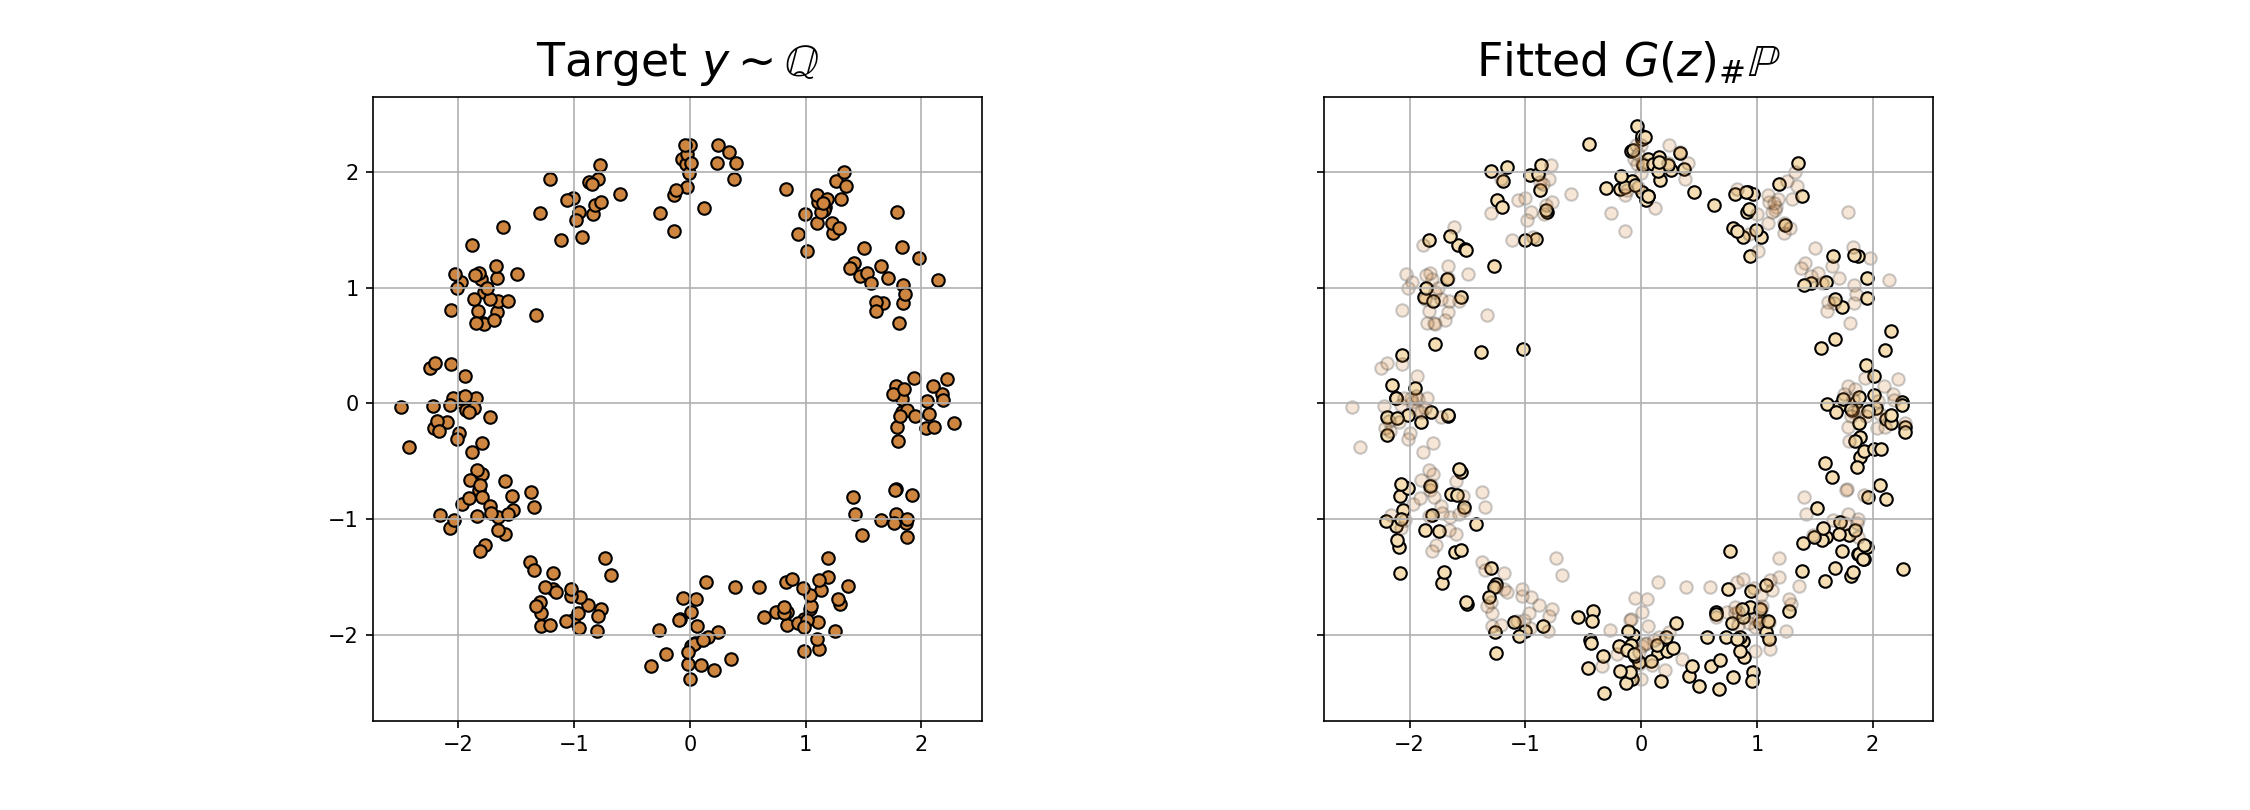
\includegraphics[width = 3in]{images/generative/2d/gaussian/12_mtd_distr.png}} &
\subfloat[Clusterization]{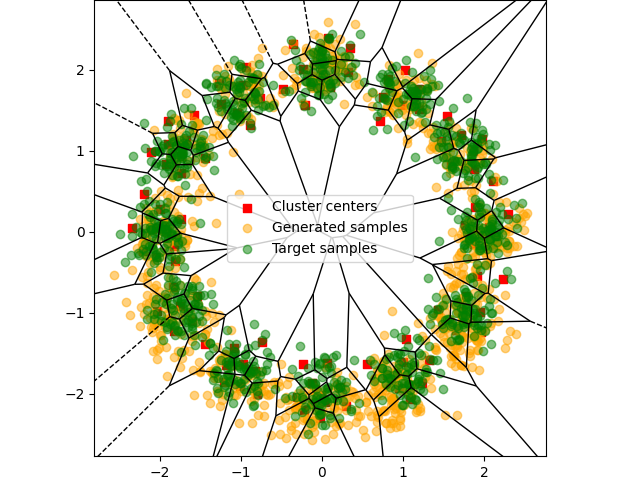
\includegraphics[width = 1.5in]{images/generative/2d/gaussian/12_mtd_ndb.png}} &
\subfloat[Precision-Recall curve]{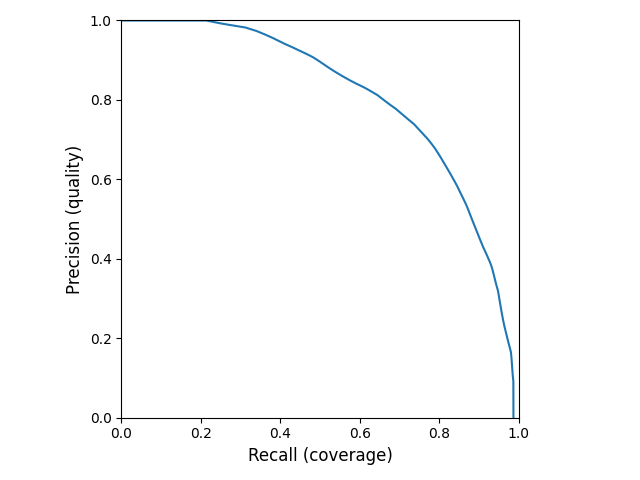
\includegraphics[width = 1.5in]{images/generative/2d/gaussian/12_mtd_prd.png}} \\
\end{tabular}
\caption{12 Gaussians + MTop-Div${}_0$}
\end{figure}



\begin{figure}[h!]
\begin{tabular}{ccc}
\subfloat[Generative sample]{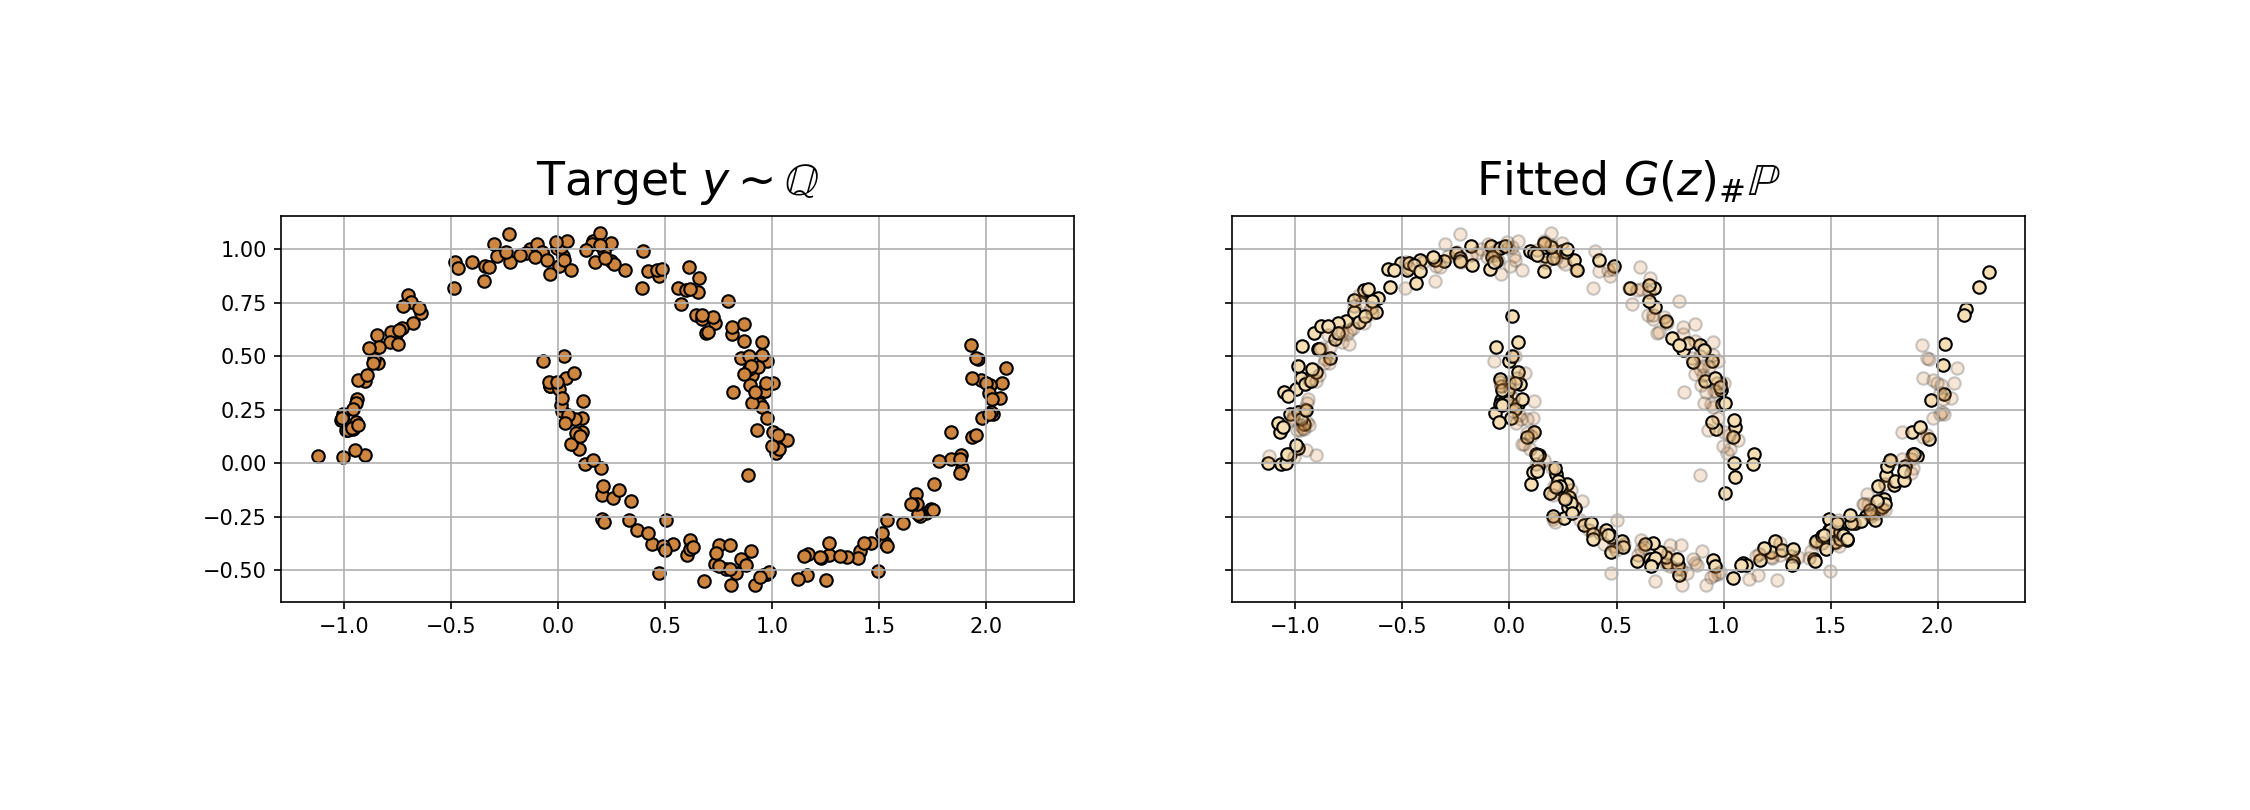
\includegraphics[width = 3in]{images/generative/2d/moons/mtd_distr.png}} &
\subfloat[Clusterization]{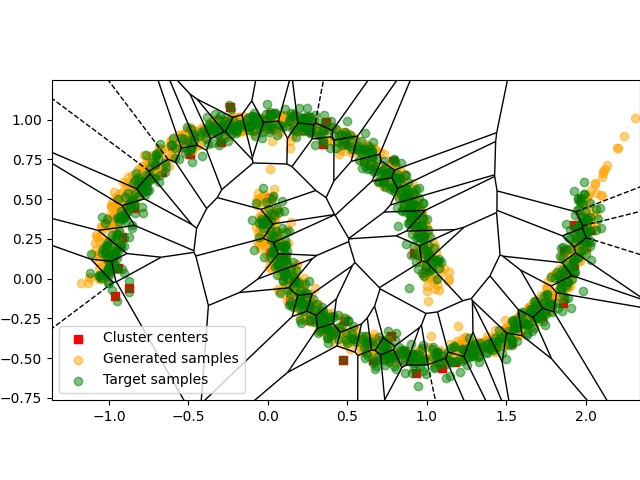
\includegraphics[width = 1.5in]{images/generative/2d/moons/mtd_ndb.png}} &
\subfloat[Precision-Recall curve]{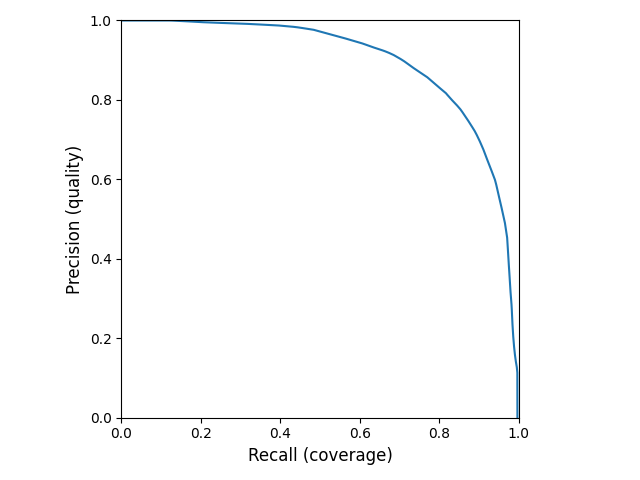
\includegraphics[width = 1.5in]{images/generative/2d/moons/mtd_prd.png}} \\
\end{tabular}
\caption{Moons + MTop-Div${}_0$}
\end{figure}



\begin{figure}[h!]
\begin{tabular}{ccc}
\subfloat[Generative sample]{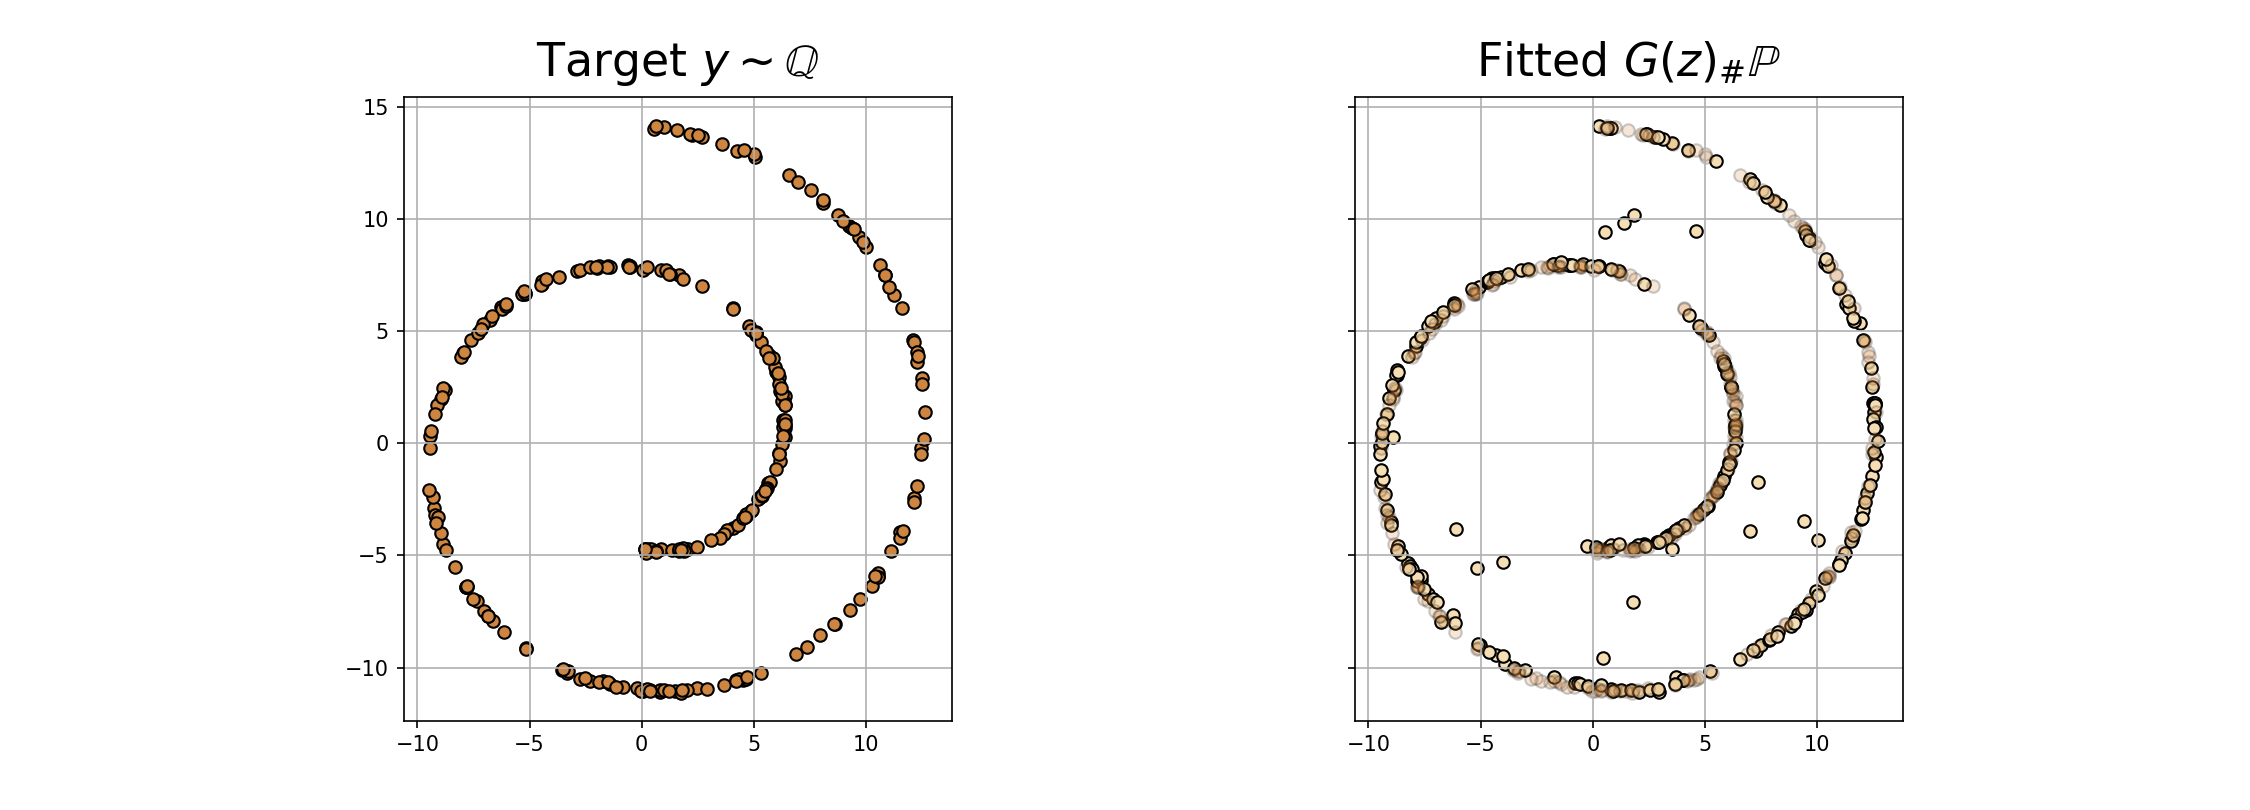
\includegraphics[width = 3in]{images/generative/2d/roll/mtd_distr.png}} &
\subfloat[Clusterization]{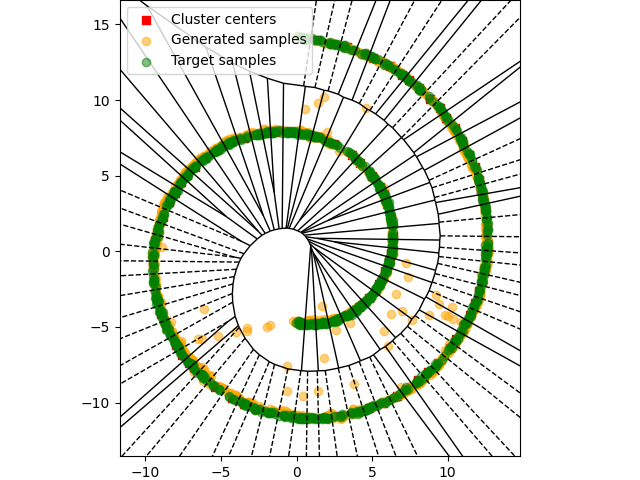
\includegraphics[width = 1.5in]{images/generative/2d/roll/mtd_ndb.png}} &
\subfloat[Precision-Recall curve]{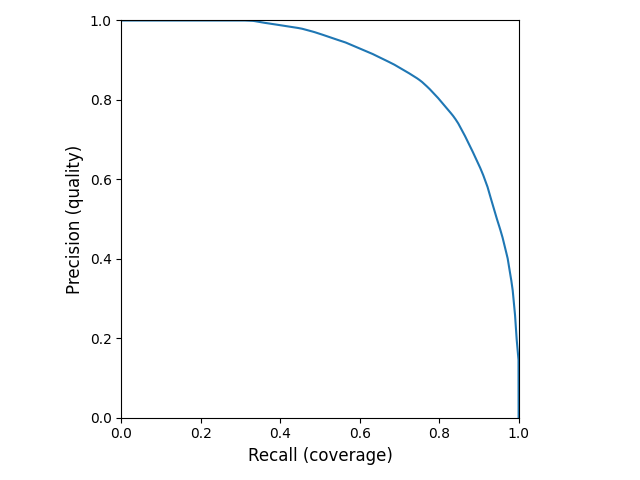
\includegraphics[width = 1.5in]{images/generative/2d/roll/mtd_prd.png}} \\
\end{tabular}
\caption{Swiss Roll + MTop-Div${}_0$}
\end{figure}


\begin{figure}[h!]
\begin{tabular}{ccc}
\subfloat[Generative sample]{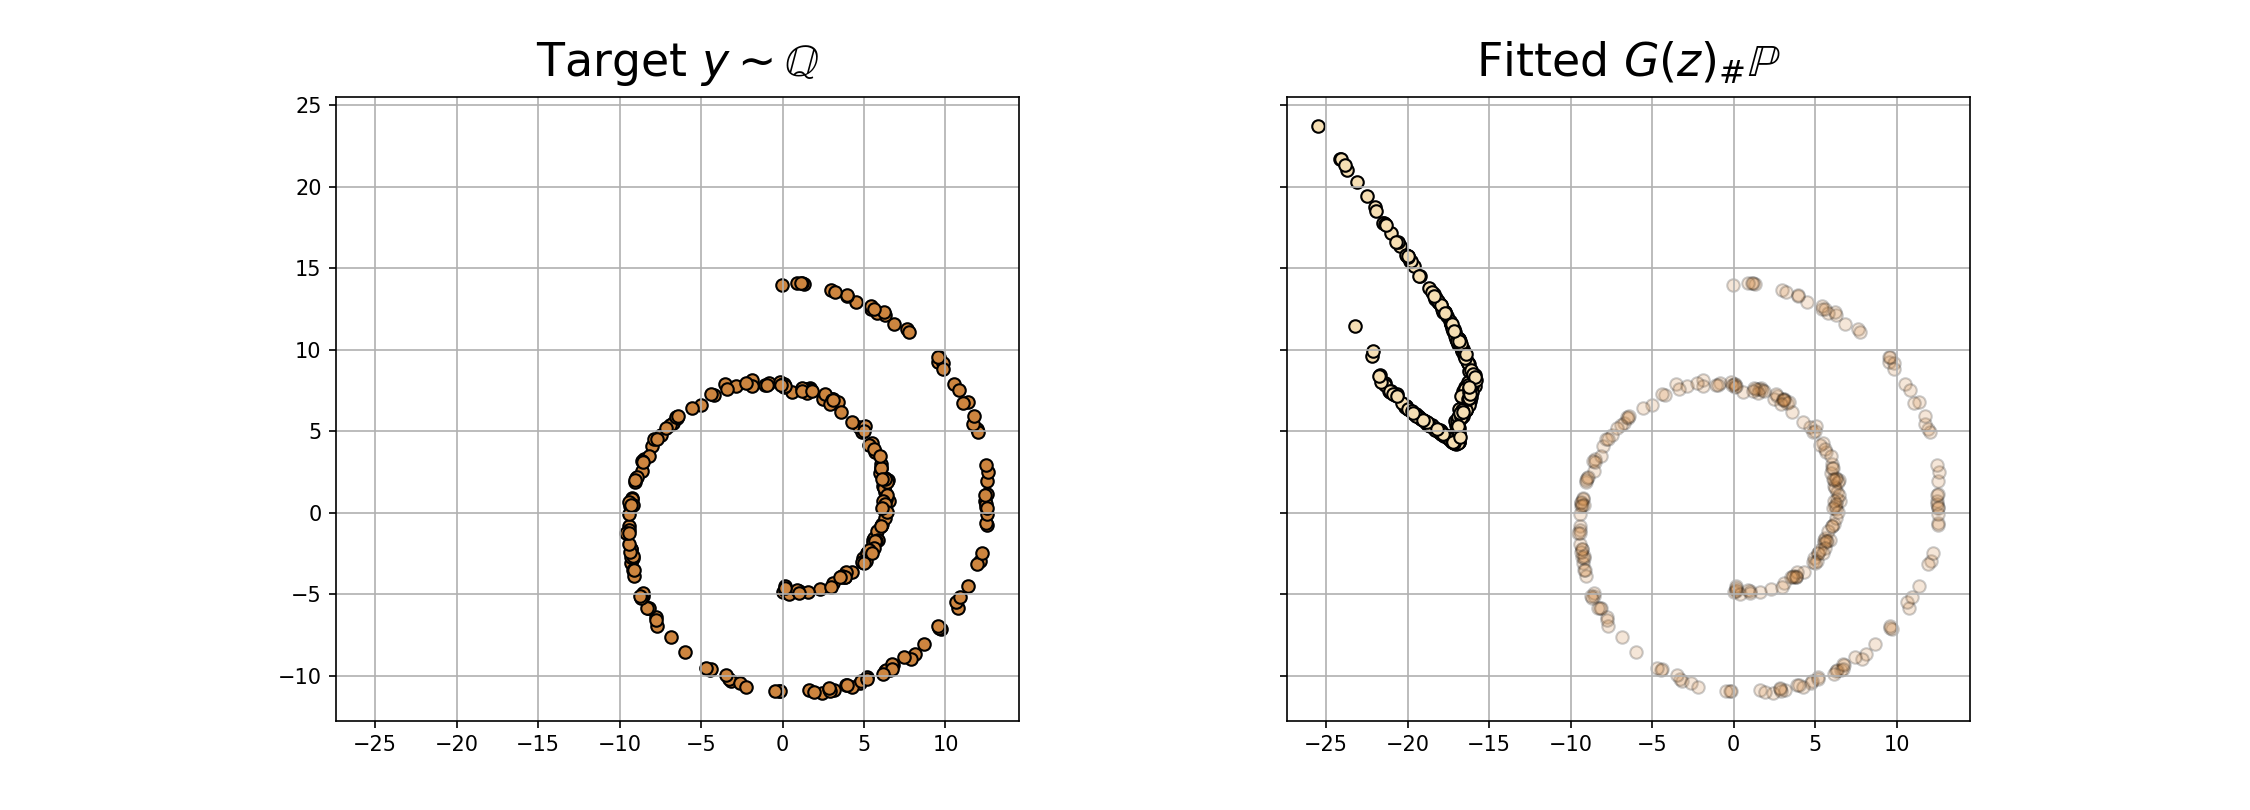
\includegraphics[width = 3in]{images/generative/2d/roll/gan_distr.png}} &
\subfloat[Clusterization]{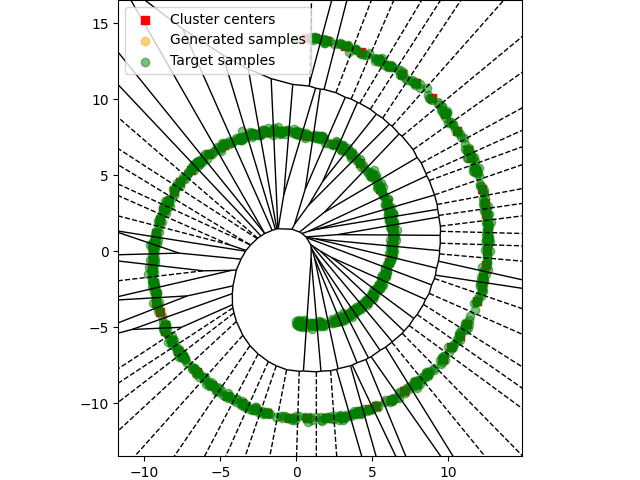
\includegraphics[width = 1.5in]{images/generative/2d/roll/gan_ndb.png}} &
\subfloat[Precision-Recall curve]{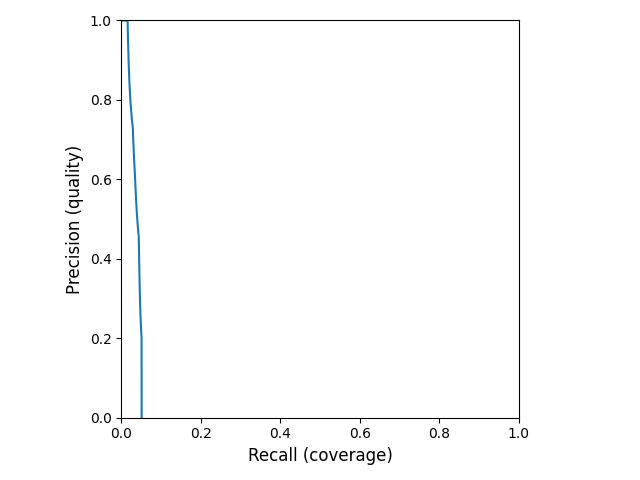
\includegraphics[width = 1.5in]{images/generative/2d/roll/gan_prd.png}} \\
\end{tabular}
\caption{Swiss Roll + Wasserstein GAN with gradient penalty displays very poor performance}
\end{figure}
\subsection{Images}
Image generation capabilities are quantified for two classical datasets: MNIST \cite{mnist} and CelebA \cite{celeba}. Note that due to high dimensionality of CelebA images we resorted to using combination of gan and topology losses on perceptual features as just MTop-Div${}_0$ is no longer sufficient to capture high-fidelity details.
For MNIST dataset we compute histograms along with Kolmogorov distance over generated class labels to verify diverse but high quality sampling. For CelebA we report Frechet Inception Distance as it is a standard metric for comparing generative models. However it does not examine sample diversity thoroughly.
\begin{figure}[h!]
\begin{tabular}{ccc}
\subfloat[MTop-Div${}_0$ samples]{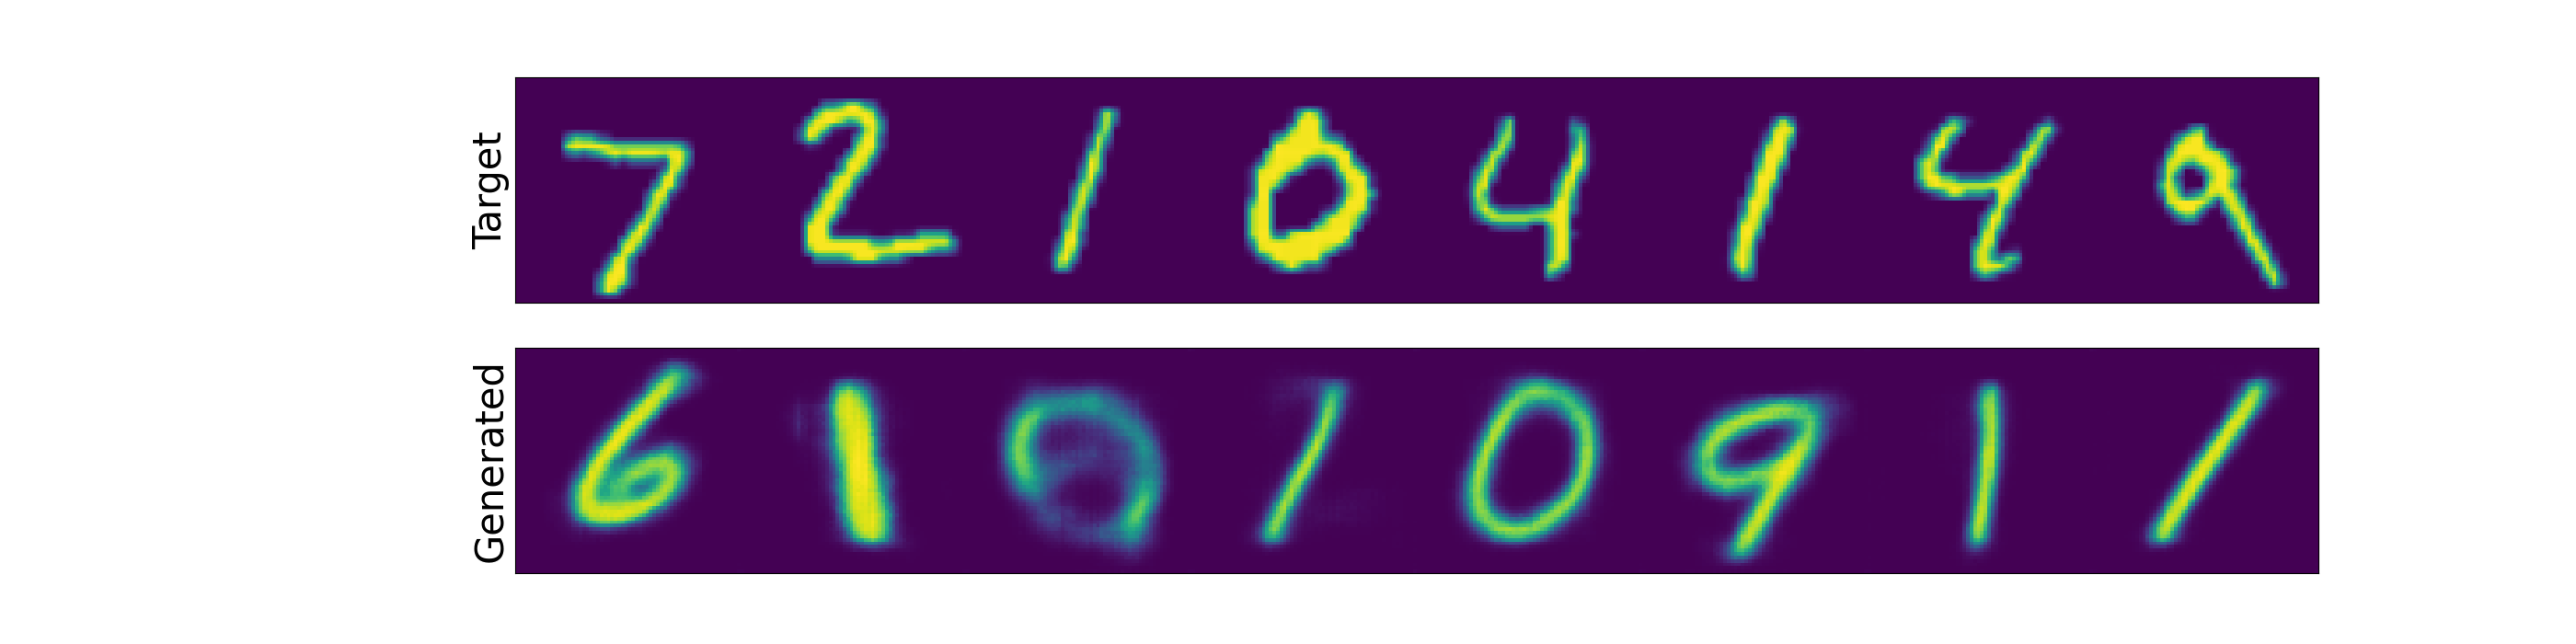
\includegraphics[width = 3in]{images/generative/images/mnist/mtd_samples.png}} & \subfloat[Histogram of MTop-Div${}_0$ labels]{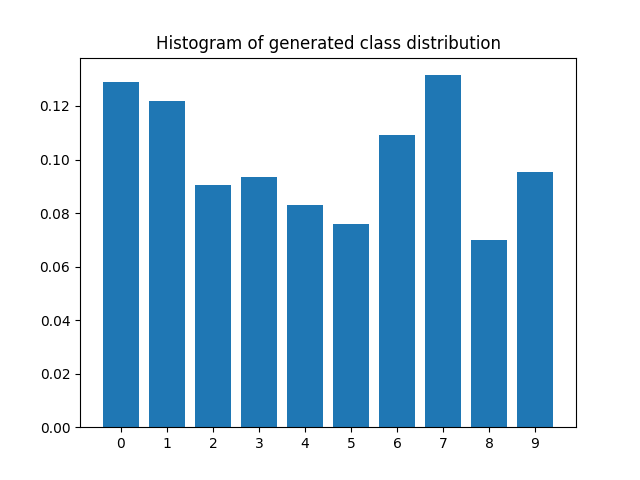
\includegraphics[width = 1.5in]{images/generative/images/mnist/media_images_class distribution_7099_f2626772ec333b941601.png}} & \subfloat[Precision-Recall curve]{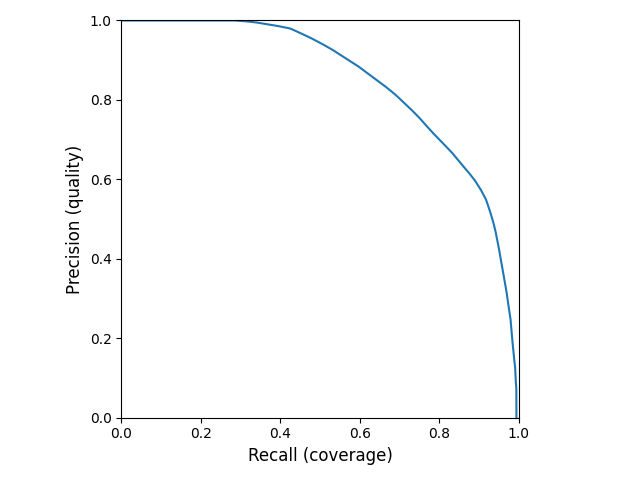
\includegraphics[width = 1.5in]{images/generative/images/mnist/mtd_prd.png}}\\
\subfloat[WGAN-GP samples]{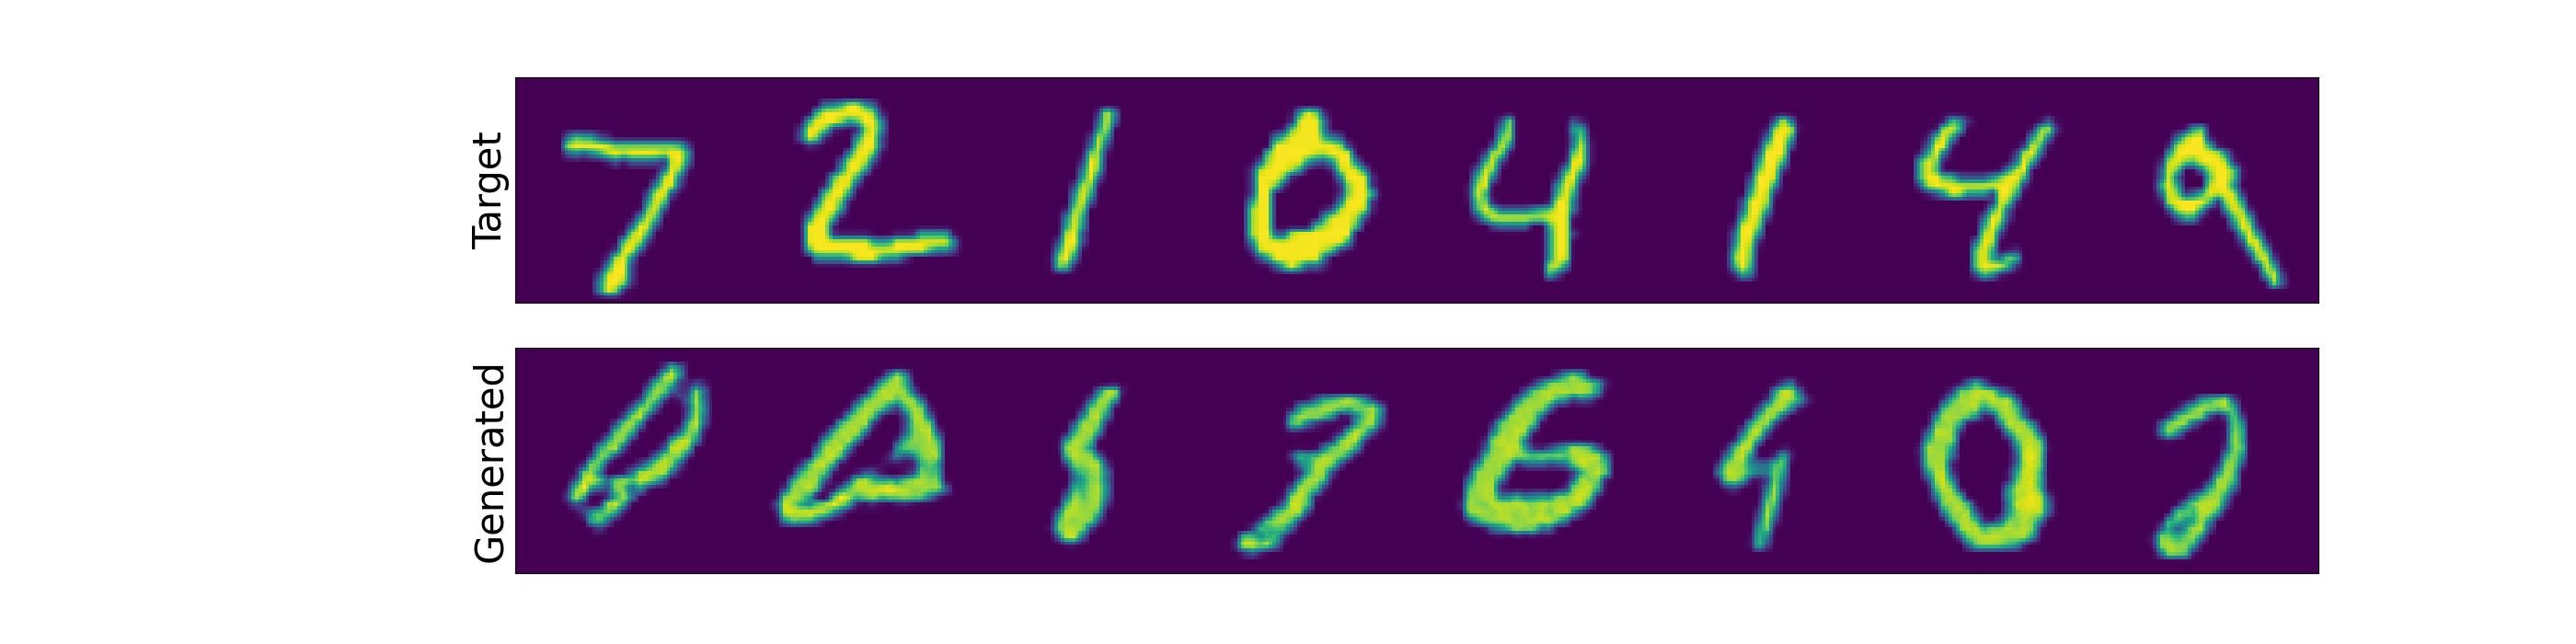
\includegraphics[width = 3in]{images/generative/images/mnist/gan_samples.png}} & \subfloat[Histogram of WGAN-GP labels]{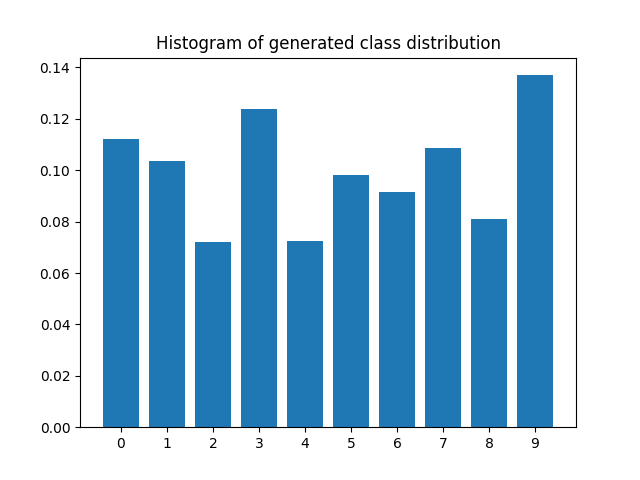
\includegraphics[width = 1.5in]{images/generative/images/mnist/gan_label_distribution.png}} & \subfloat[Precision-Recall curve]{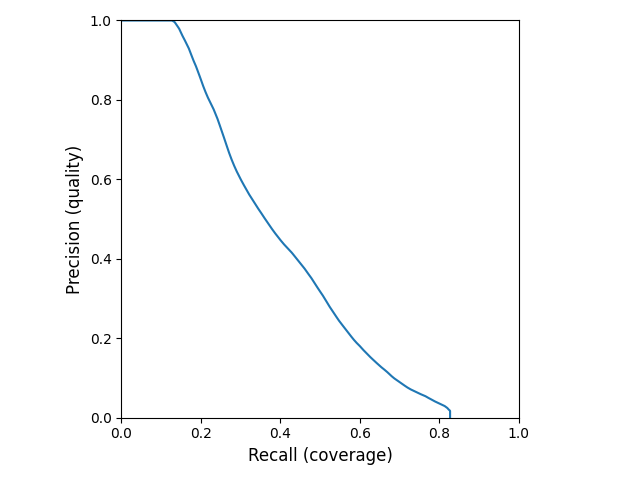
\includegraphics[width = 1.5in]{images/generative/images/mnist/media_images_precision recall_35462_e1abe8f2ceea4017daa5.png}} \\
\subfloat[Example of mode collapse in GAN training]{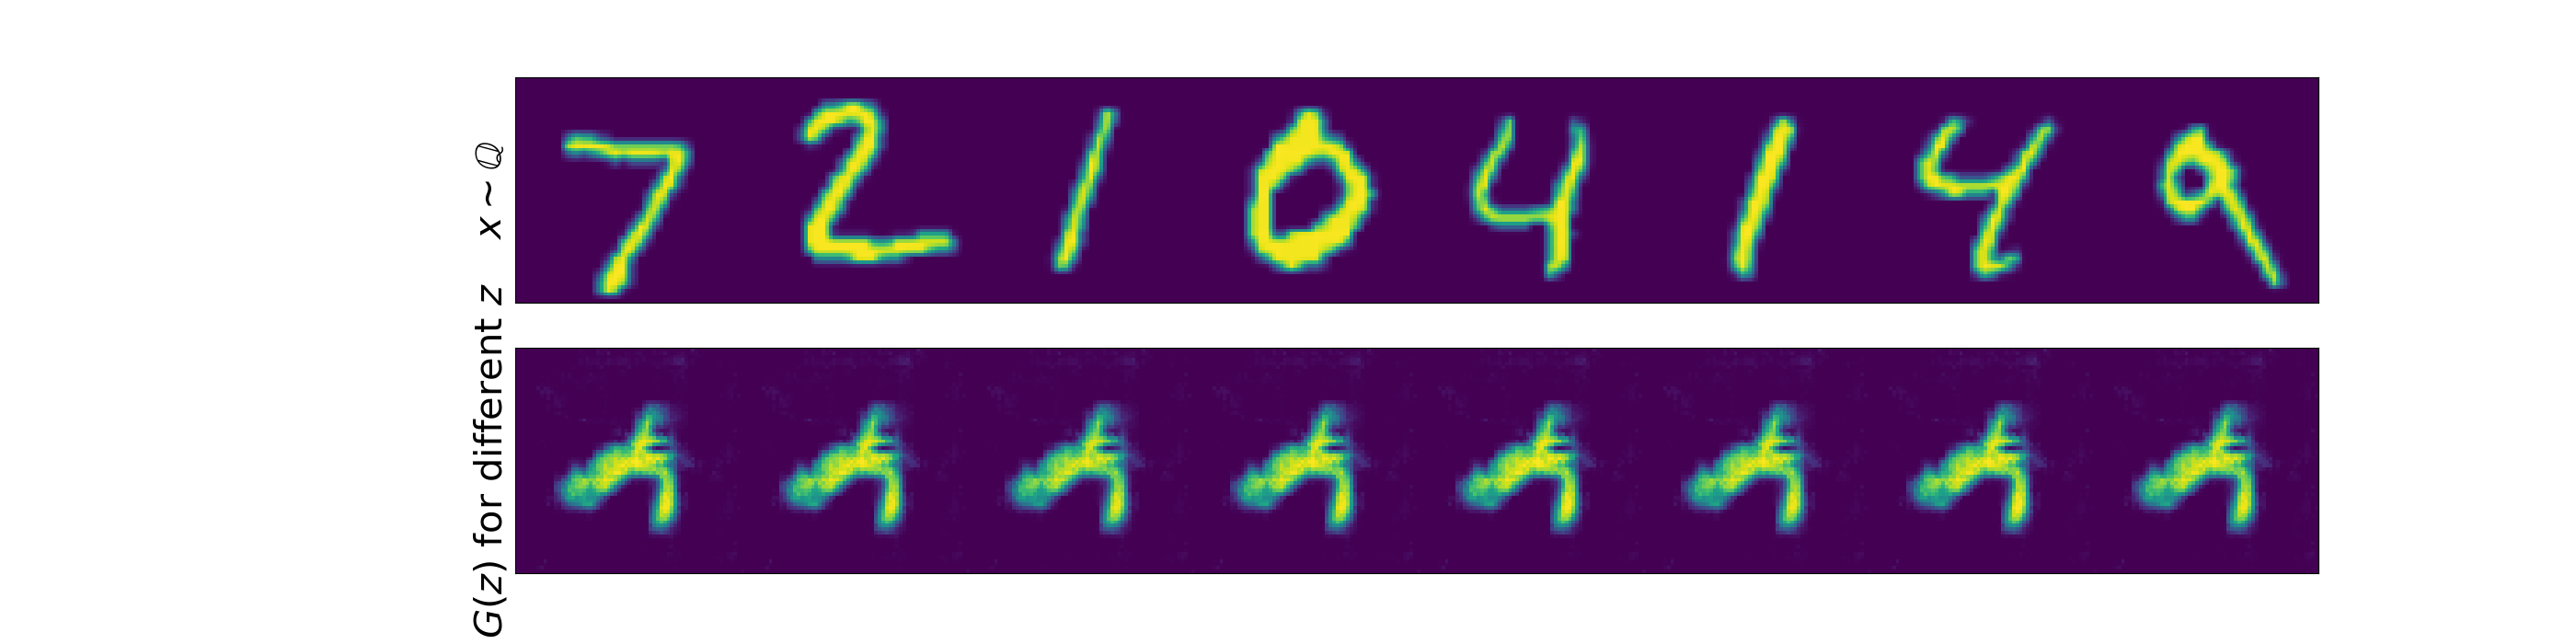
\includegraphics[width = 3in]{images/generative/images/mnist/example_of_mode collapse_in_GAN.png}} & & \\
\end{tabular}
\caption{MNIST samples}
\end{figure}

\begin{table}[h!]
    \centering
    \begin{tabular}{||c||c|c|c|c|c||}
        \hline \hline
         Method  & NDB ratio $\downarrow$& JS $\downarrow$ & max$F_1$ $\uparrow$ & TVD $\downarrow$ & Kolm. dist. w. uniform $\downarrow$\\ \hline \hline
         WGAN-GP   & 0.68 & 0.247 & 0.422 & 0.577 & 0.037 \\ \hline
         MTop-Div${}_0$   & \textbf{0.32} & \textbf{0.046} & \textbf{0.753} & \textbf{0.247} & \textbf{0.0315} \\ \hline 
        \hline
    \end{tabular}
    \caption{Best metrics for MNIST dataset}
    \label{tab:my_label}
\end{table}

\begin{figure}[h!]
\begin{tabular}{cc}
\subfloat[MTop-Div${}_0$ samples]{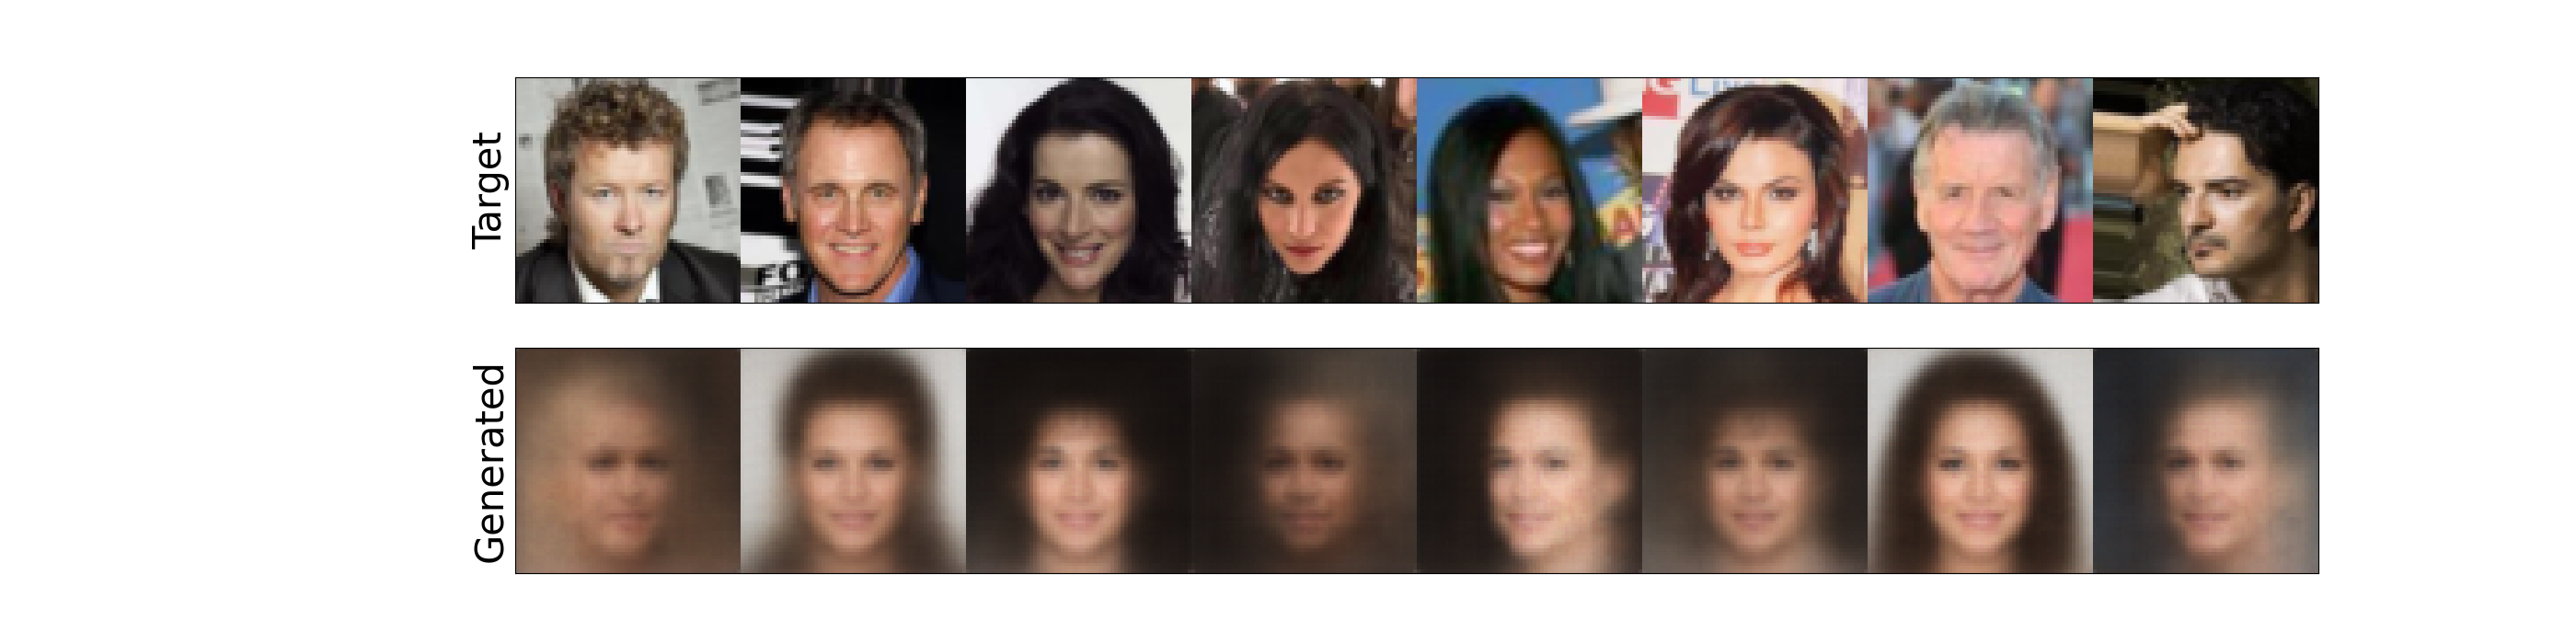
\includegraphics[width = 3in]{images/generative/images/celeba/mtd.png}} & \subfloat[Precision-Recall curve]{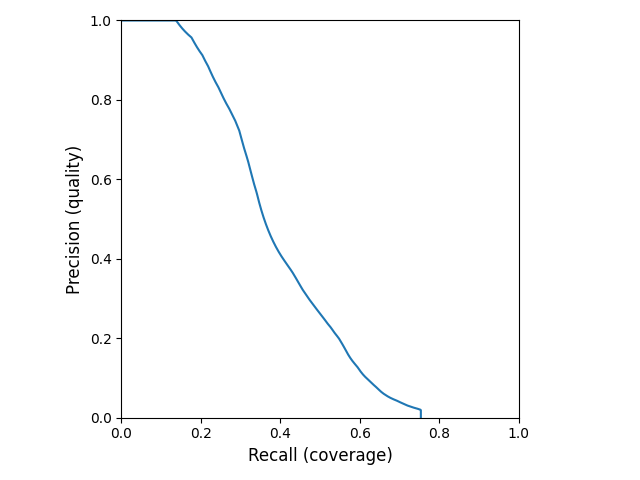
\includegraphics[width = 1.5in]{images/generative/images/celeba/mtd_pr.png}}\\
\subfloat[WGAN-GP samples]{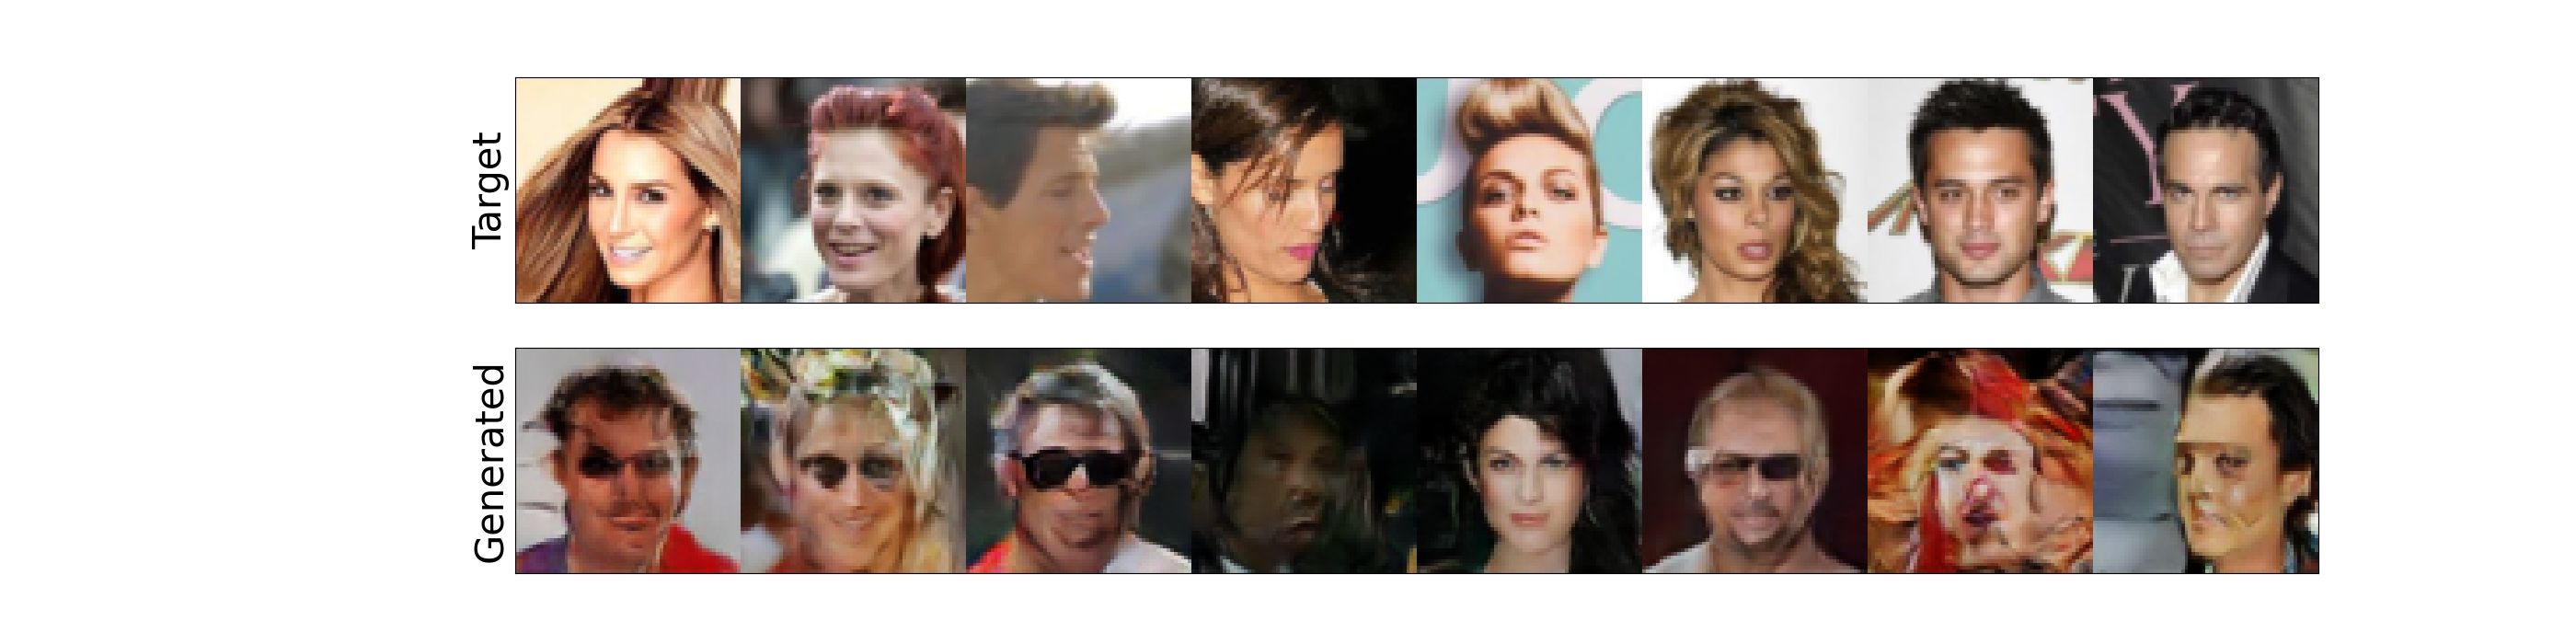
\includegraphics[width = 3in]{images/generative/images/celeba/gan.png} \label{fig:glasses}} & \subfloat[Precision-Recall curve]{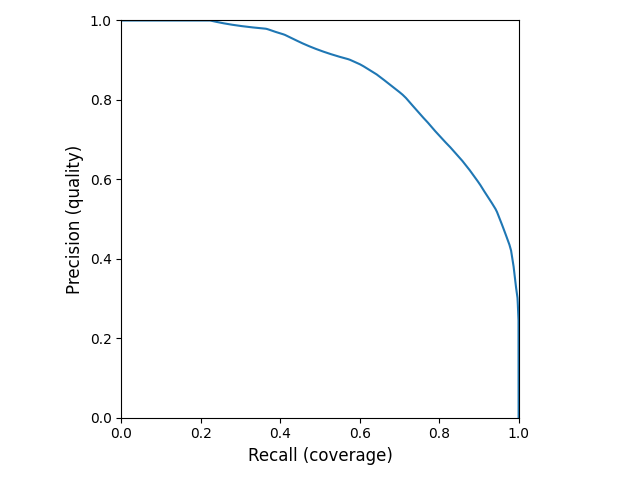
\includegraphics[width = 1.5in]{images/generative/images/celeba/gan_pr.png}} \\
\subfloat[WGAN-GP with MTop-Div${}_0$ reg.]{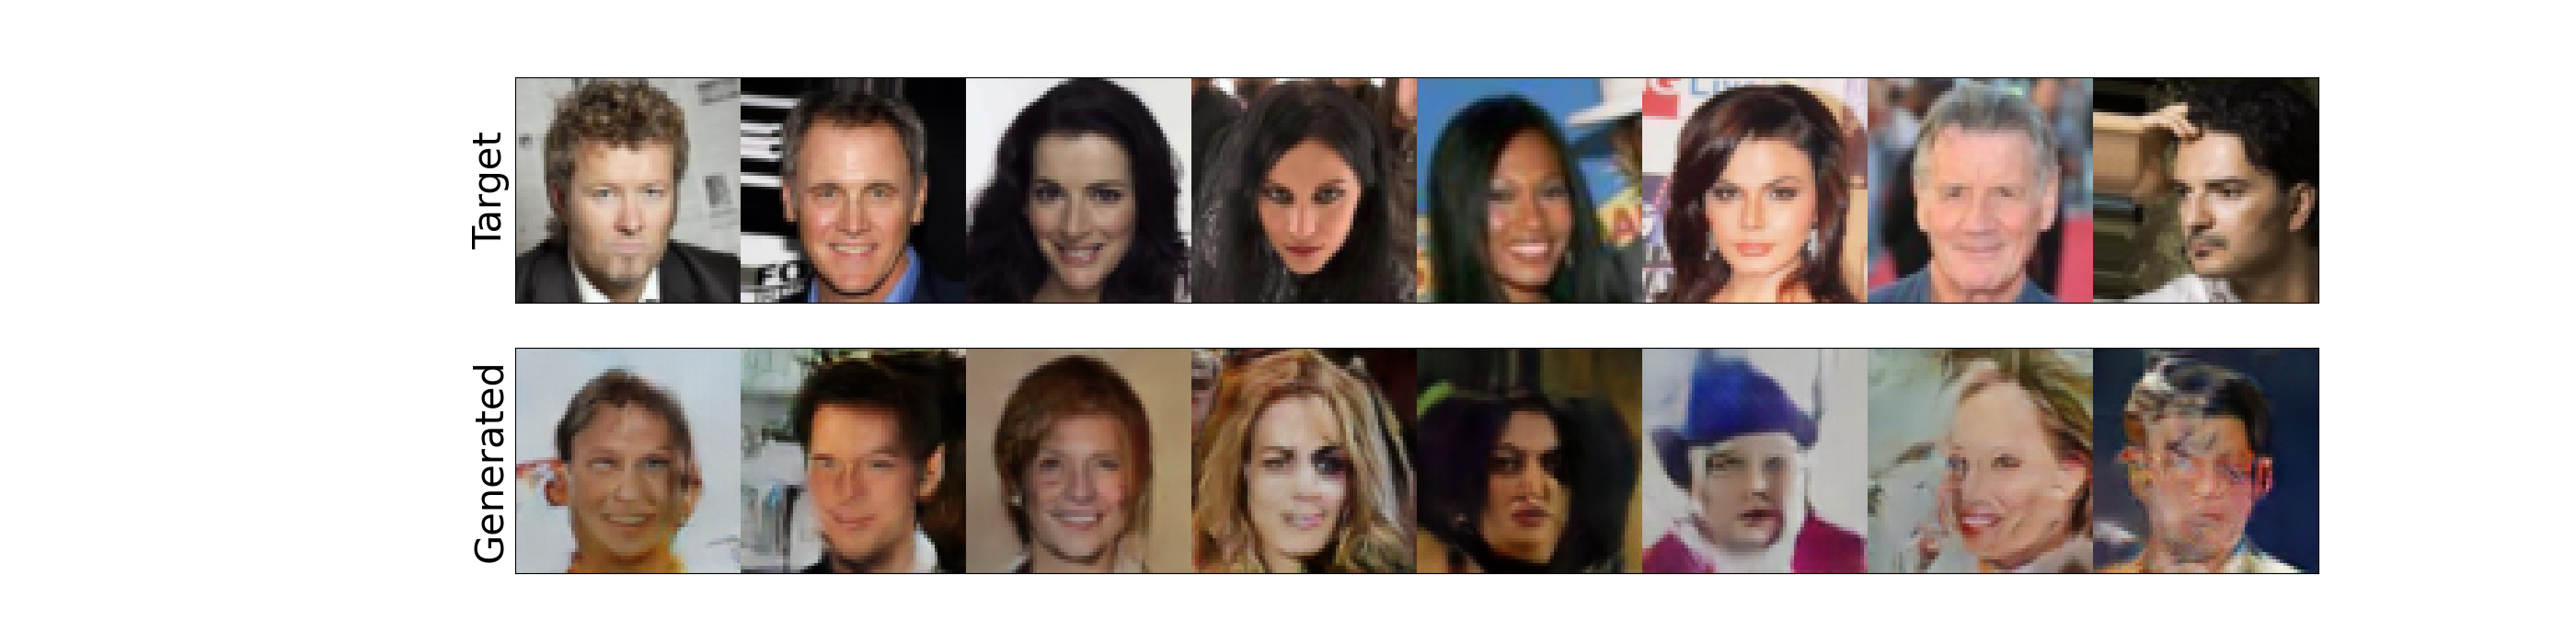
\includegraphics[width = 3in]{images/generative/images/celeba/gan_mtd.png}} & \subfloat[Precision-Recall curve]{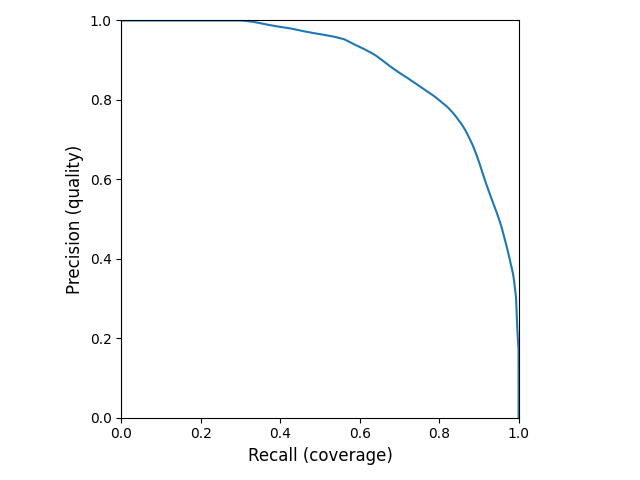
\includegraphics[width = 1.5in]{images/generative/images/celeba/gan_mtd_pr.png}} \\
\end{tabular}
\caption{CelebA samples}
\end{figure}

\begin{table}[h!]
    \centering
    \begin{tabular}{||c||c|c|c|c|c||}
        \hline \hline
         Method  & NDB ratio $\downarrow$& JS $\downarrow$ & max$F_1$ $\uparrow$ & TVD $\downarrow$ & FID $\downarrow$\\ \hline \hline
         WGAN-GP   & 0.41 & 0.043 & 0.759 & 0.242 & 0.319 \\ \hline
         MTop-Div${}_0$   & 0.8 & 0.255 & 0.427 & 0.596 & 1.549 \\ \hline 
         WGAN-GP+MTop-Div${}_0$   & \textbf{0.36} & \textbf{0.033} & \textbf{0.801} & \textbf{0.2} & \textbf{0.313} \\ \hline 
        \hline
    \end{tabular}
    \caption{Best metrics for CelebA dataset}
    \label{tab:my_label}
\end{table}
It is immediately obvious that usage of MTop-Div${}_0$ is superior across almost all comparisons. And in case of CelebA dataset it improves quality and diversity yet again (notice how many generated samples from WGAN-GP have glasses \ref{fig:glasses} indicating high concentration in particular mode).

\section{3D reconstruction experiments}
We use three Mip-NeRF-360 scenes, namely, bicycle, bonsai and garden to compare algorithm \ref{algo:reg} with standard Gaussian Splatting fitting algorithm by means of proposed metric.

\begin{table}[h!]
    \centering
    \begin{tabular}{||c||c|c|c||}
    \hline \hline
        {} & bicycle & bonsai & garden \\
    \hline \hline
        LGCR without regularizer $\downarrow$ & 58.82 & \textbf{66.67} & 27.03 \\
        \hline
        LGCR with regularizer $\downarrow$ & \textbf{46.51} & 125 & \textbf{23.54} \\
    \hline \hline
    \end{tabular}
    \caption{LGCR metric values for different scenes with or without regularizer}
    \label{tab:my_label}
\end{table}

\begin{figure}
    \centering
    \includegraphics[width=\textwidth]{images/gaussian/Screenshot 2024-05-30 at 14.53.51.png}
    \caption{Example of reconstructed Gaussian field for scene 'train' from original paper}
    \label{fig:train}
\end{figure}

\begin{figure}
    \centering
    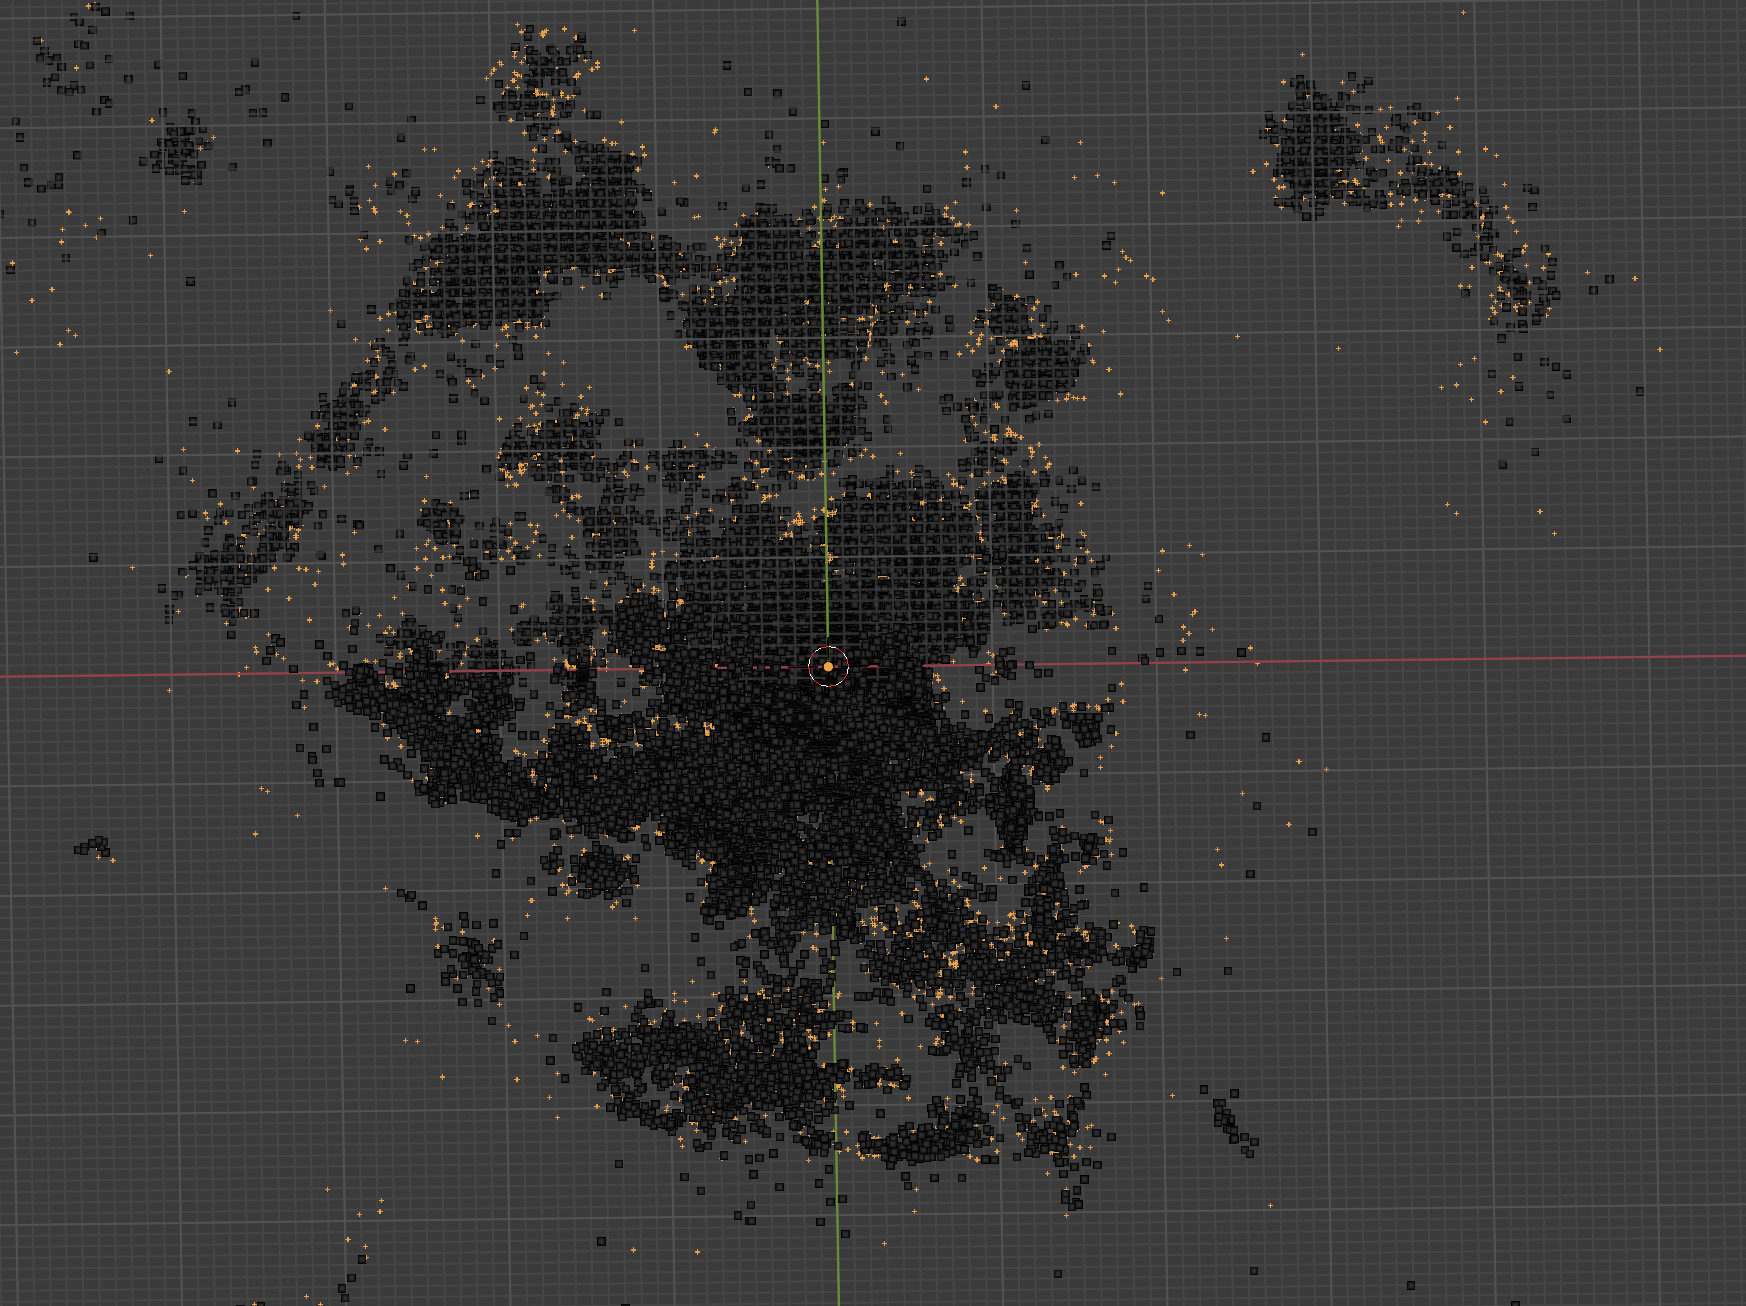
\includegraphics[width=\textwidth]{images/gaussian/Screenshot 2024-06-04 at 03.08.28.png}
    \caption{Many floaters and spurious vertices in reconstruction of 'bonsai'}
    \label{fig:train}
\end{figure}
Unfortunately values of proposed metric are hard to compare across different scenes, because number of large-scale cluster heavily depends on type of scene (indoor/outdoor), presence of opaque substances, quality of Structure-from-motion initialization and other things. We at least detect improvement in two out of three scenes, and will look for ways to make this method more performant and feasible to compute.

